% To do:
% aaai12's paper (not important)

\begin{figure}[tb!]
\begin{center}
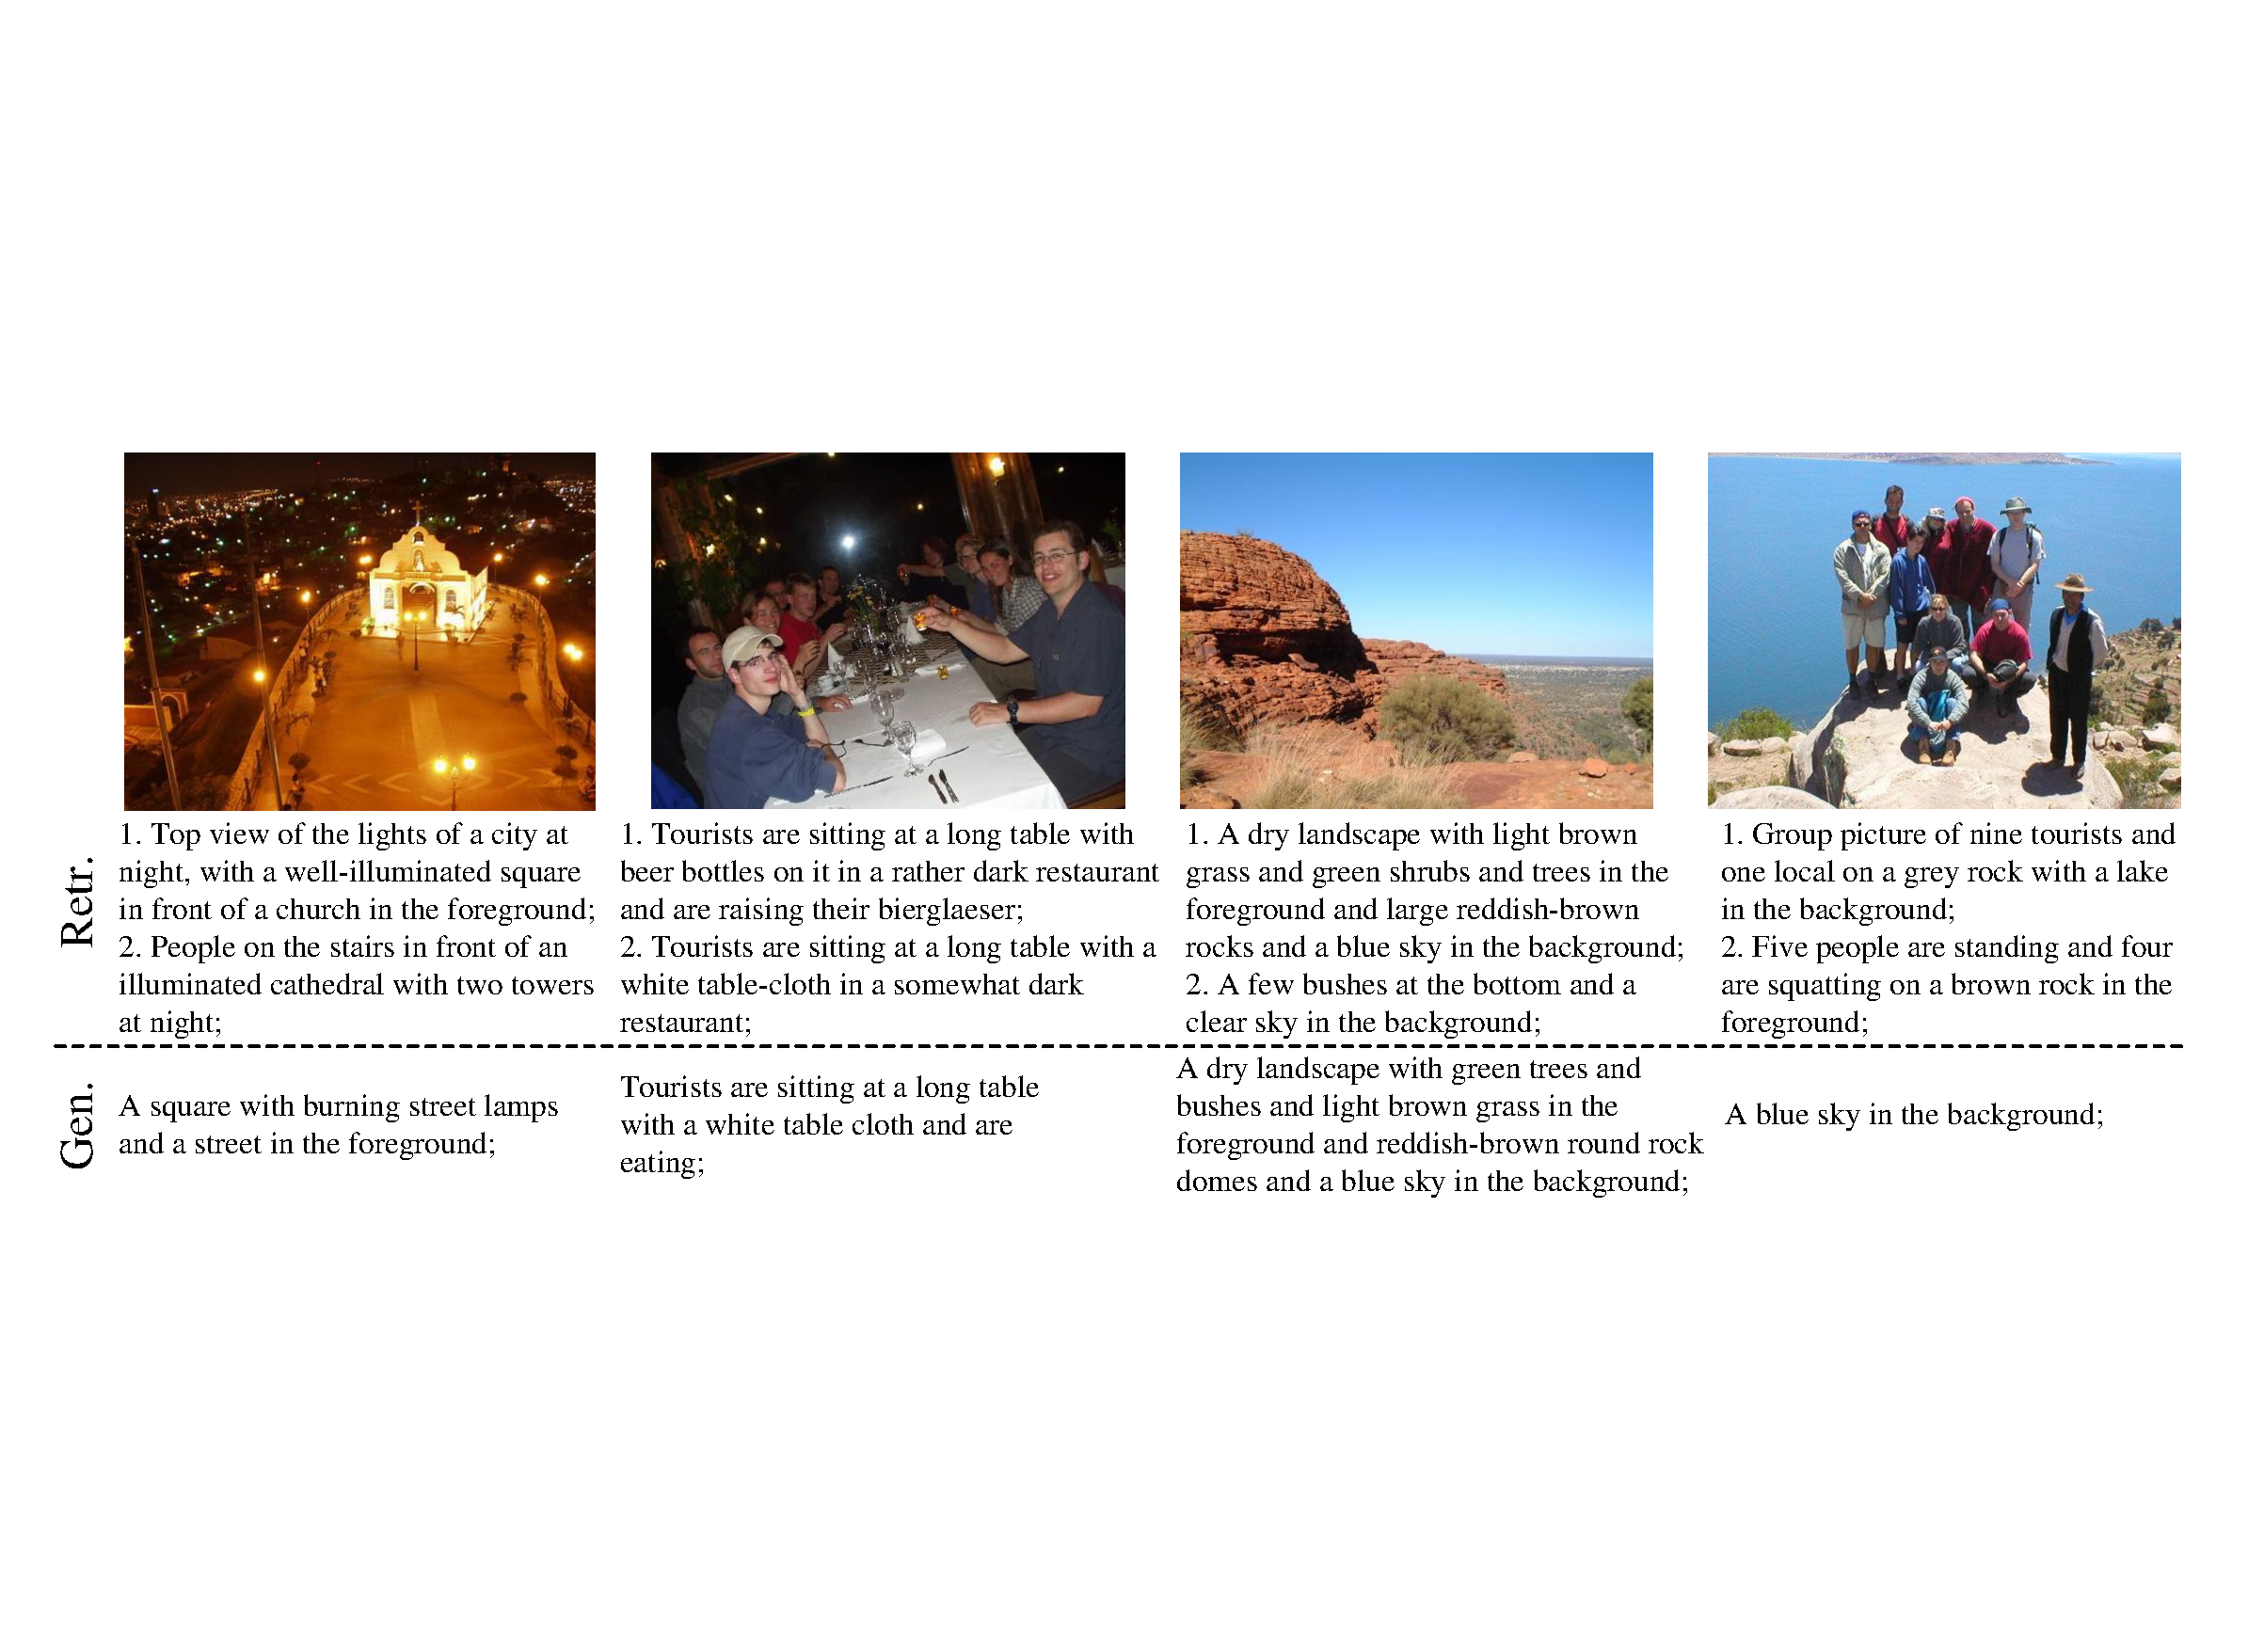
\includegraphics[width=0.98\linewidth]{PaperFigures/res_example.pdf}
\end{center}
   \caption{Examples of the generated and two top-ranked retrieved sentences given the query image from IAPR TC-12 dataset.
   The sentences can well describe the content of the images.
   We show a failure case in the fourth image, where the model mistakenly treats the lake as the sky.
   }
\label{fig:res_example}
\end{figure}

\section{Related Work}
\label{sec:related_work}

\textbf{Deep model for computer vision and natural language.}
The deep neural network structure develops rapidly in recent years in both the field of computer vision and natural language.
For computer vision, Krizhevsky et. al \cite{krizhevsky2012imagenet} proposed a deep convolutional neural networks with 8 layers (denoted as AlexNet) for image classification tasks and outperformed previous methods by a large margin.
Recently, Girshick et. al \cite{girshick2014rcnn} proposed a object detection framework based on AlexNet.
For natural language, the Recurrent Neural Network shows the state-of-the-art performance in many tasks, such as speech recognition and word embedding learning \cite{mikolov2010recurrent,mikolov2011extensions,mikolov2013distributed}.

\textbf{Image-sentence retrieval.}
Many works treat the task of describe images as a retrieval task and formulate the problem as a ranking or embedding learning problem \cite{hodosh2013framing,frome2013devise,socher2014grounded}.
They will first extract the word and sentence features (e.g. Socher et.al \cite{socher2014grounded} uses dependency tree Recursive Neural network to extract sentence features) as well as the image features.
Then they optimize a ranking cost to learn an embedding model that maps both the language feature and the image feature to a common semantic feature space.
In this way, they can directly calculate the distance between images and sentences.
Most recently, Karpathy et.al \cite{karpathy2014fragment} showed that object level image features based on object detection results will generate better results than image features extracted at the global level.

\textbf{Generating novel sentence descriptions for images.}
There are generally two categories of methods for this task.
The first category assumes a specific rule of the language grammar.
They parse the sentence and divide it into several parts \cite{mitchell2012midge,gupta2012image}.
Then each part is associated to a object or an attribute in the image (e.g. \cite{kulkarni2011baby} uses a Conditional Random Field model and \cite{farhadi2010every} uses a Markov Random Field model).
This kind of method generates sentences that are syntactically correct.
Another category of methods, which is more related to our method, learns a probability density over the space of multimodal inputs (i.e. sentences and images), using for example, Deep Boltzmann Machines \cite{srivastava2012multimodal}, and topic models \cite{barnard2003matching,jia2011learning}.
They can generate sentences with richer and more flexible structure than the first group.
The probability of generating sentences given the corresponding image can serves as the affinity metric for retrieval.
Our method falls into this category.
More close related to our tasks and method is the work of Kiros et al. \cite{kiros2013multimodal}, which is built on a Log-BiLinear model \cite{mnih2007three}.
It needs a fixed length of context (i.e. five words), whereas in our model, the temporal context is stored in a recurrent architecture, which allows arbitrary context length.
